% Template for ICASSP-2019 paper; to be used with:
%          spconf.sty  - ICASSP/ICIP LaTeX style file, and
%          IEEEbib.bst - IEEE bibliography style file.
% --------------------------------------------------------------------------
\documentclass{article}
\usepackage{spconf,amsmath,graphicx}
\usepackage{color,amsfonts}

% Example definitions.
% --------------------
\def\x{{\mathbf x}}
\def\L{{\cal L}}

% Title.
% ------
\title{Nonparallel Emotional Speech Conversion}
%
% Single address.
% ---------------
%\name{Author(s) Name(s)\thanks{Thanks to XYZ agency for funding.}}
%\address{Author Affiliation(s)}
%
% For example:
% ------------
%\address{School\\
%	Department\\
%	Address}
%
% Two addresses (uncomment and modify for two-address case).
% ----------------------------------------------------------
%\twoauthors
%  {A. Author-one, B. Author-two\sthanks{Thanks to XYZ agency for funding.}}
%	{School A-B\\
%	Department A-B\\
%	Address A-B}
%  {C. Author-three, D. Author-four\sthanks{The fourth author performed the work
%	while at ...}}
%	{School C-D\\
%	Department C-D\\
%	Address C-D}
%

\name{Jian Gao $^{\star}$ \qquad Deep Chakraborty $^{\dagger}$ \qquad Olaitan Olaleye $^{\ddagger}$}
\address{$^{\star}$ Department of Computer Science and Engineering, New York University, USA \\ $^{\dagger}$ College of Information and Computer Sciences, University of Massachusetts, Amherst, USA \\ $^{\ddagger}$ Affiliation Number Three}


\begin{document}
%\ninept
%
\maketitle
%
\begin{abstract}
We propose a nonparallel data-driven emotional speech conversion framework. The goal is to change emotion-related characteristics of a speech signal while preserving the speaker identity and linguistic content. Most existing approaches require parallel data and time alignment, which is not only tedious work to prepare the data but also a source of quality degradation due to misalignment. We achieve nonparallel training based on an unsupervised style transfer technique, which learns a translation model between two distributions instead of a deterministic one-to-one mapping between paired data. The translation model consists of a encoder and a decoder for each emotion domain. We assume that the speech signal can be decomposed into an emotion-invariant content code and an emotion-related style code in some latent space. Emotion conversion is performed by recombining the content code of the source speech and the style code of the desired emotion. We tested our method on a nonparallel corpora with four emotions. Both subjective and objective evaluations show the effectiveness of our approach.
%This model consists of an autoencoder with a generative adversarial network and is trained with weak cycle consistency loss, adversarial loss, and reconstruction loss
\end{abstract}

%
\begin{keywords}
Emotional speech conversion, nonparallel data, style transfer, autoencoder, GAN
\end{keywords}
%



\section{Introduction}
\label{sec:intro}
Voice transformation (VT) is a technique to modify some properties of human speech while preserving its linguistic information. VT can be applied to change the speaker identity, i.e., voice conversion (VC) [1], or to transform the speaking style of a speaker, such as emotion and accent conversion [2]. In this work, we will focus on voice transformation for emotional speech. The goal is to change emotion-related characteristics of a speech signal while preserving its linguistic content and speaker identity. Emotion conversion techniques can be applied to various tasks ({\color{blue} need one sentence, and references})

Traditional VC approaches cannot be directly applied because they change speaker identity by assuming pronunciation and intonation to be a part of the speaker-independent information. Since the speaker's emotion is mainly conveyed by prosodic aspects, some studies focus on modeling prosodic features such as pitch, pause, stress, tempo and volume  [3][4][5]. In [6], a rule-based emotional voice conversion system was proposed by modifying prosody-related acoustic features of neutral speech to generate different kinds of emotional speech. It uses speech analysis-synthesis tool STRAIGHT [7] to extract fundamental frequency ($F_0$) and power envelope, and then parameterize them by Fujisaki model [8] and target prediction model [9]. The modified features are then fed into STRAIGHT to re-synthesis speech waveforms with desired emotions. However, this method not only needs parallel data for training, but also requires time modification to align the speech duration of each utterance pair. The duration-related features are extracted by manual segmentation of the speech signal at phoneme level. Though this approach did successfully convert emotions, it is hard to obtain adequate time-aligned utterance pairs and also inconvenient in real applications due to the manual operation.
%On the other side, automatic time alignment algorithm like dynamic time warping (DTW) may cause performance degradation due to mismatching.
% time consuming and tedious task

%it's harder to get parallel emotional speech corpora (dataset XXX) than VC.
%need professional actors, since in normal life, it's rare to find angry sentences pronounced in a happy style
To address this issue, we propose a method for nonparallel training. Instead of learning one-to-one mapping between paired emotional utterances, we switch to training a conversion model between two emotional domains. Let $x_1 \in \mathcal{X}_1$ and $x_2 \in \mathcal{X}_2$ be utterances drawn from two different emotional categories, our model learns a mapping between two distributions $p(x_1)$ and $p(x_2)$. Since the joint distribution $p(x_1, x_2)$ is unknown, we cannot directly estimate the conversion models $p(x_1|x_2)$ and $p(x_2|x_1)$.

Inspired by disentangled representation learning in image style transfer [10], we assume that each speech signal $x_i \in \mathcal{X}_i$ can be decomposed into a content latent code $c \in \mathcal{C}$ that represents emotional-independent information and a style latent code $s_i \in \mathcal{S}_i$ that represents emotion-related information. $\mathcal{C}$ is shared across domains that contains the information we want to preserve, and $\mathcal{S}_i$ is domain specific that contains the information we want to change. In conversion stage, we extract content code of the source speech and recombine it with style code of the desired emotion. A generative adversarial network (GAN) [16] is added to improve the quality of converted speech. Our approach is nonparallel, text-independent, and does not rely on any external data, preprocessing or manual operation. The model can be trained on a small amount of utterances ($\sim$ 8 min per emotion).

%We employ gated convolutional neural networks (CNNs) [13] to model the speech representations. This allows the autoencoder to capture the long-range dependencies in speech. The conversion model is trained with a weak cycle consistency loss [14, 15], which helps to create pseudo pairs from nonparallel data. And and keep it indistinguishable from the real ones.

We evaluated our approach on IEMOCAP [17] with four emotions: angry, happy, neutral, sad.
%It is a nonparallel dataset widely used in emotional speech recognition and analysis.
An objective evaluation showed that our model can modify the speech to significantly increase the percentage of desired emotions. A subjective evaluation on Amazon MTurk showed that the converted speech had good quality and preserved the speaker identity.

The rest of the paper is organized as follows: Section \ref{sec:related} presents the relation to prior work. Section \ref{sec:method} gives a detailed description of our model. Experiment and evaluation results are reported in Section \ref{sec:exp}. Finally, we conclude in Section \ref{sec:con}.

%reviews existing work that are most closely related to our approach
% pairwise transformation function

\section{Related Work}
\label{sec:related}

\subsection{Emotion-related features}
Previous emotion conversion methods directly modify parameterized prosody-related features that convey emotions. [11] first proposed to use Gaussian mixture models (GMM) for spectrum transformation. [12] introduced a data-driven emotion conversion system that combines independent parameter transformation techniques including HMM-based $F_0$ generation, $F_0$ segment selection, duration conversion and GMM-based spectral conversion. However, it requires large amounts of parallel data.

A recent work [6] explored four types of acoustic features: $F_0$ contour, spectral sequence, duration and power envelope, and investigated their impact on emotional speech synthesis by controlled feature replacement. They found that $F_0$ and spectral sequence are the dominant factors in emotion conversion, while power envelope and duration alone has little influence. They further claimed that all emotions can be synthesised by modifying the spectral sequence, but they did't know how to do it. In this paper, we focus on learning the conversion models for $F_0$ and spectral sequence. Since changing duration and power envelope requires manually segmenting the phoneme boundaries of vowels and consonants, we leave it for future work.

\subsection{Nonparallel training approaches}
%In parallel setting, the training data is limited to a small amount of predefined sentences, which may impair the generalization ability.
%It is a time consuming and painstaking task to collect parallel data. Training on well-aligned parallel data is easy, but collecting such data is hard.
Parallel data means utterances with the same linguistic content but vary in aspects to be studied. Since parallel data is hard to collect, nonparallel approaches have been developed. Some borrow ideas from image-to-image translation and create models suitable for speech, such as VAE-based SC [22], VC-VAW-GAN [18], VC-CycleGAN [20][21] and VC-StarGAN [25]. Another trend is to use WaveNet architecture [23], which is an autoregressive model for raw audio synthesis. Although it can generate high-quality speech, the huge amount of computation resource and training data is not affordable for most users.

%Our approach only needs a small amount of training data ($\sim$ 8 min per emotion), and does not rely on any transcripts, manual operation, or preprocessing step.
%Our method differs in that; external data

\subsection{Disentangled representation learning}
Our work draws inspiration from recent studies in image style transfer. A basic idea is to find disentangled representations that can independently model image content and style. It is claimed in [10] that Convolutional Neural Network (CNN) is an ideal representation to factorize semantic content and artistic style. They introduced a method to separate and recombine content and style of natural images by matching feature correlations in different convolutional layers. For us, the task is to find disentangled representations for speech signal that can split emotion from speaker identity and linguistic content.


%factorize variations in object identity and its precise appearance.
%learning disentangled representations for speech.
%factorise the variation in the content of an image and the variation in its appearance
%claimed the image content and style information are separable in Convolutional Neural Network representations
%find image representations that independently model variations in the semantic image content and the style

% a small amount of expressive training data (∼15 min) and which have been evaluated for three target emotions: anger, surprise and sadness.
%such as speech rate, voice quality and fundamental frequency ($F_0$).
%In rule-based synthesis systems, fuzzy inference system acts as connectors to learn the non-linear rules between desired emotions and acoustic features.

%match the target styles
% It reports the important of four types of prosodic parameters:

\section{Method}
\label{sec:method}

\subsection{Assumptions}
%Emotions are nonlinguistic information not generally controlled by speakers.
The research of human emotion expression and perception has two major conclusions.
First, human emotion perception is a multi-layered process. For example, [26] figured out that humans do not perceive emotion directly from acoustic features, but through an intermediate layer of semantic primitives. They introduced a three-layered model and built the connections by a fuzzy inference system. Some researchers found that adding middle layer can improve the emotion recognition accuracy. Based on this finding, we suggest to use multilayer perceptron (MLP) to encode emotion-related information in speech.

Second, the emotion production of human speech follows the opposite direction of emotion perception. This means the encoding process of the speaker is the inverse operation of the decoding process of the listener. We assume that emotion speech production and perception share the same representation methodology, {\color{blue} therefore the encoder and the decoder have mirror structures.}

Define $\mathcal{X}_i$ as the speech domain with emotion $i$. Given parallel data, we can draw sample pairs $(x_1, x_2)$ from the joint distribution $P(x_1, x_2)$, $x_1 \in \mathcal{X}_1, x_2 \in \mathcal{X}_2$. It is easy to learn the conditions $P(x_2|x_1), P(x_1|x_2)$. However, nonparallel data only give us the marginal distributions $P(x_1)$ and $P(x_2)$. Since estimating the joint distribution from marginal distribution is an ill-posed problem, additional conditions are required. We assume that the speech signal can be decomposed into a domain-invariant content code and a domain-dependent style code.

Fig. \ref{autoencoder} shows the generative model of speech with a partially shared latent space. A pair of corresponding speech $(x_1, x_2)$ is assumed to have a shared latent code $c \in \mathcal{C}$ and emotion-related style codes $s_1 \in \mathcal{S}_1, s_2 \in \mathcal{S}_2$. For any emotional speech $x_i$, we have a deterministic decoder $x_i = G_i(c_i,s_i)$ and its inverse encoders $c_i = E_i^c(x_i)$, $s_i = E_i^s(x_i)$. To convert emotion, we just recombine the content code of the source speech with the style code of the target emotion.
\begin{equation}
\begin{aligned}
x_{1\leftarrow2}' = G_1(c_2, s_1) = G_1(E_2^c(x_2), s_1) \\
x_{2\leftarrow1}' = G_2(c_1, s_2) = G_2(E_1^c(x_1), s_2)
\end{aligned}
\end{equation}
It should be noted that the style code $s_i$ is not inferred from one utterance, but learnt from the entire emotion domain. Because the emotion style from a single utterance is ambiguous and may not capture the general character of the target emotion. This makes our assumption slightly different from the cycle consistent constraint [19]. When an utterance is converted to another emotion and converted back, it does not need to be exactly the same as the original signal, i.e., $x_{1\leftarrow2\leftarrow1}'' \neq x_1$. Instead, we apply the cycle-consistency in the shared latent space by assuming that $E_1^c(x_{1\leftarrow2}') = c_1$.

\begin{figure}[htb]
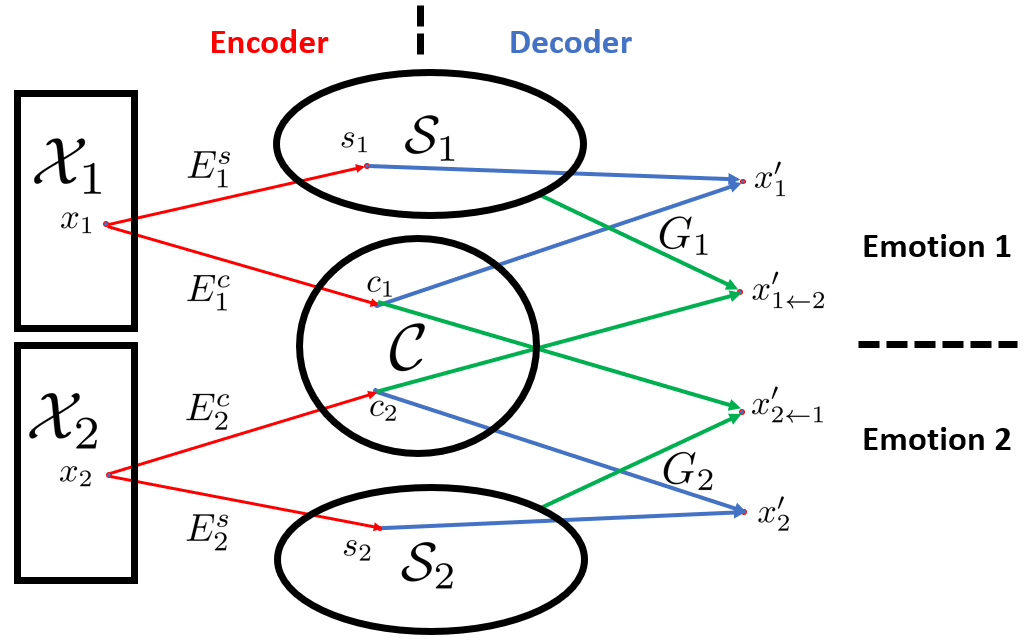
\includegraphics[width=0.48\textwidth]{FIG/autoencoder}
\caption{Speech autoencoder model with partially shared latent space. Utterance with emotion $i$ is decomposed into a emotion-dependent space $\mathcal{S}_i$ and a shared content space $\mathcal{C}$. Emotion conversion is conducted by recombining the content code of the input utterance and the style code randomly sampled from the target emotion space.}
\label{autoencoder}
\end{figure}


\subsection{Model}
% ignore the treasures in computer music before the age of deep learning.
Traditional emotional speech analysis mainly works on four types of acoustic features: fundamental frequency ($F_0$), spectral sequence, time duration and energy envelope. It was found in [6] that only $F_0$ and spectral sequence have significant influence, while the other two require manual segmentation and have little impact on changing the emotions. Therefore we focus on learning the conversion model for $F_0$ and spectral sequence. Fig. \ref{model} shows an overview of our nonparallel emotional speech conversion system. The acoustic features are extracted and recombined by WORLD analysis system [27] and converted separately.

We convert $F_0$ by linear transform to match statistics of the fundamental frequencies in the target emotion domain. The conversion is performed by logarithm Gaussian normalization
\begin{equation}
f_2 = \exp((\log f_1 - \mu_1)\cdot\frac{\sigma_2}{\sigma_1} + \mu_2)
\label{eq:f0}
\end{equation}
where $\mu_i, \sigma_i$ are the mean and variance obtained from the target emotion set. Aperiodicity (AP) is mapped directly since it does not contain emotion-related information.

\begin{figure}[htb]
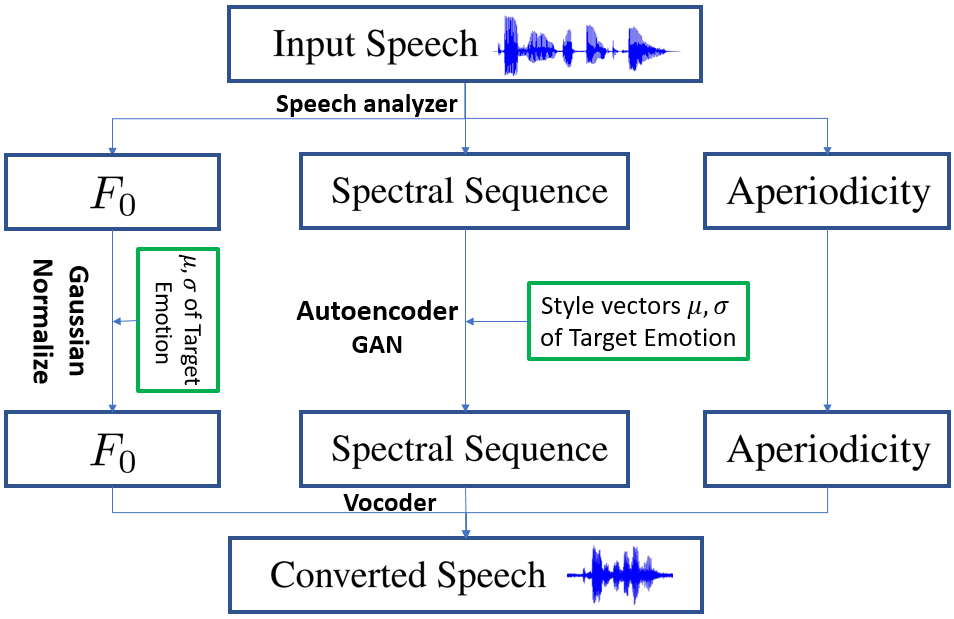
\includegraphics[width=0.48\textwidth]{FIG/model}
\caption{Overview of nonparallel emotion conversion system}
\label{model}
\end{figure}

For spectral sequence, we use low-dimensional representation in mel-cepstrum (MCEP) domain to reduce computation complexity. [28] shows that 50 MCEP coefficients are enough to synthesize full-band speech without quality degeneration. Spectra conversion is learnt by the autoencoder model in Fig. \ref{autoencoder}. The encoders and decoders are implemented with gated convolutional neural networks [13]. In addition, two generative adversarial networks (GANs) were added to produce realistic spectral frames. Our model has 4 subnetworks $E^c, E^s, G, D$, in which $D$ is the discriminator in GANs to distinguish between real samples and machine-generated samples.


\subsection{Loss functions}
We jointly train the encoders, decoders and GAN's discriminators with multiple losses displayed in Fig. \ref{loss}. To keep encoder and decoder as inverse operations, we apply reconstruction loss in the direction $x_i \rightarrow (c_i, s_i) \rightarrow x_i'$. The spectral sequence should not change after encoding and decoding.
\begin{equation}
L_{recon}^{x_i} = \mathbb{E}_{x_i}(\| x_i - x_i' \|_1), \quad x_i' = G_i(E_i^c(x_i), E_i^s(x_i))
\end{equation}

\begin{figure}[htb]
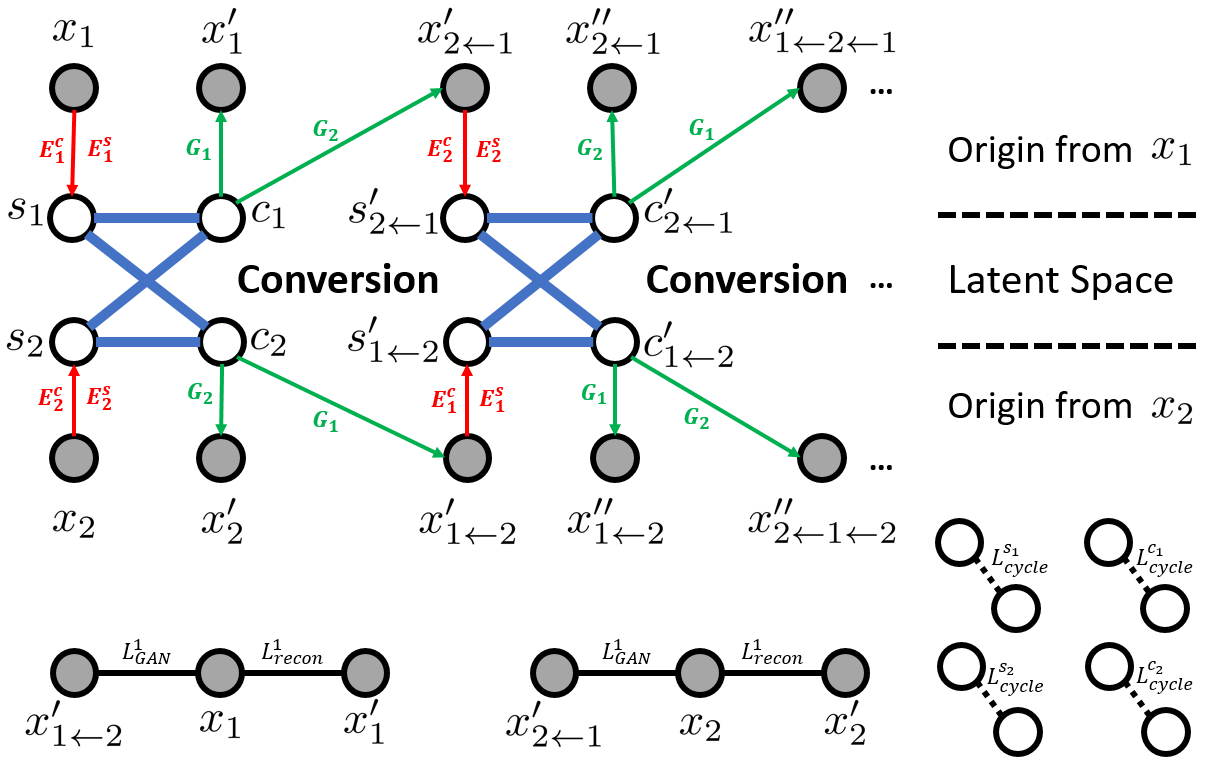
\includegraphics[width=0.48\textwidth]{FIG/loss}
\caption{Train on multiple loss functions}
\label{loss}
\end{figure}
%$x_1, x_2, x_1', x_2'$
%$s_1, c_1, s_2, c_2$ \\
%$c_{1\leftarrow2}', s_{1\leftarrow2}', c_{2\leftarrow1}', s_{2\leftarrow1}'$ \\
%$x_{2\leftarrow1}', x_{1\leftarrow2}', x_{2\leftarrow1}'', x_{1\leftarrow2}''$ \\
%$x_{1\leftarrow2\leftarrow1}'', x_{2\leftarrow1\leftarrow2}''$

In our model, the latent space is partially shared. Thus the cycle consistency constraint [19] is not preserved, i.e., $x_{1\leftarrow2\leftarrow1}'' \neq x_1$. We apply a semi-cycle loss in the coding direction $c_1 \rightarrow x_{2\leftarrow1}' \rightarrow c_{2\leftarrow1}'$ and $s_2 \rightarrow x_{2\leftarrow1}' \rightarrow s_{2\leftarrow1}'$.
\begin{equation}
\begin{aligned}
L_{cycle}^{c_1} = \mathbb{E}_{c_1, s_2} (\| c_1 - c_{2\leftarrow1}' \|_1), \quad c_{2\leftarrow1}'=E_2^c(x_{2\leftarrow1}') \\
L_{cycle}^{s_2} = \mathbb{E}_{c_1, s_2} (\| s_2 - s_{2\leftarrow1}' \|_1), \quad s_{2\leftarrow1}'=E_2^s(x_{2\leftarrow1}')
\end{aligned}
\end{equation}

Moreover, we add a GAN module to improve the speech quality. The converted samples should be indistinguishable from the real samples in the target emotion domain. GAN loss is computed between $x_{i\leftarrow j}'$ and $x_i$, $(i \neq j)$.
\begin{equation}
L_{GAN}^i = \mathbb{E}_{c_j, s_i}[\log(1-D_i(x_{i\leftarrow j}'))] + \mathbb{E}_{x_i}[\log D_i(x_i)]
\end{equation}
The full loss is the weighted sum of $L_{recon}$, $L_{cycle}$, $L_{GAN}$.
\begin{equation}
\begin{aligned}
\min_{E_1^c,E_1^s,E_2^c,E_2^s, G_1,G_2}\max_{D_1,D_2} L(E_1^c, E_1^s, E_2^c, E_2^s, G_1, G_2, D_1, D_2) \\
= \lambda_s (L_{cycle}^{s_1} + L_{cycle}^{s_2}) + \lambda_c (L_{cycle}^{c_1} + L_{cycle}^{c_2}) \ \qquad \qquad \\
+ \lambda_x (L_{recon}^1 + L_{recon}^2) + \lambda_g (L_{GAN}^1 + L_{GAN}^2) \qquad \quad
\end{aligned}
\end{equation}
where $\lambda_s, \lambda_c, \lambda_x, \lambda_g$ control the weights of the components.
%1. reconstruction loss: ensures the encoders and decoders are inverse functions
%
%2. cycle-consistency loss in the latent space
%
%3. generative adversarial loss: produce realistic spectral frames


%, emotion is encoded as "distal indicator cues". A listener perceives the cues through a middle procedure called “proximal percepts”, and then use those percepts to recognize emotions. Similarly, in the three-layered model, there's a middle layer called "semantic primitive" between the emotion layer and acoustic feature layer. People found adding the middle layer can improve emotion recognition accuracy.

%, i.e., the encoding process of the speaker is the inverse decoding process of the listener




%we assume that the human production of emotion follows the opposite direction of human perception. This means the encoding process of the speaker is the inverse process of the decoding of the listener.

%Brunswik’s model suggests that the process of perception of emotion is multi-layered.
%the procedure of human emotion perception is a multiplelayered process.

%The three-layered model has already been applied by some researchers in the emotion recognition area
%In this paper, the voice conversion system for emotional speech is built with a single speaker.

% we use a multi-layer perception (MLP) to learn emotion.
% 17 semantic primitives used in the three-layered model
% emotion recognition: 3 layer model is better, VGG

%Both Brunswik’s functional lens model and the three-layered model are used to account for human emotion perception. According to Juslin who also uses the Brunswik’s lens model in Juslin (2000), two important conclusions can be made: firstly, speakers can communicate emotions successfully to listeners, and secondly, the cue utilization of speakers maps well to the cue utilization of listeners. This indicates that speakers and listeners share the same representation methodology (i.e., coding method) when doing vocal communication. According to this result, we assume that human production of emotion is the mirror effect of human perception of emotions which means the encoding process of the speaker is the inverse process of the decoding process of the listener.

%The autoencoder is implemented in CNN with gated activation to capture both temporal structure and spectral texture
%Wasserstein GAN loss [xx] was used to generate more realistic spectral shapes.



\section{Experiments}
\label{sec:exp}

\subsection{Corpus}
We test the proposed method on IEMOCAP [17], which is a widely used corpus for emotion recognition. To our knowledge, this is the first work to use it for emotion conversion. IEMOCAP contains scripted and improvised
dialogs in five sessions; each has labeled emotional sentences pronounced by two English speakers. The emotions in scripted dialogs have strong correlation with the lingual content. Since our task is to change emotion but keep the speaker identity and linguistic content, we only use the improvised dialogs of the same speaker. We train the conversion model on four emotions: angry, happy, neutral, sad. The acoustic features $F_0$, spectral sequence and AP are extracted by WORLD [27] every $5$ ms, then coded to $24$-dimension Mel-cepstral vectors of temporal size $128$ as the autoencoder's input.

%It has background noise, close to real applications. Collect data from YouTube


\subsection{Network Architecture}
Our network structure is illustrated in Fig. \ref{fig:NN}. The encoders and decoders are implemented with one-dimension CNNs to capture the temporal dependencies; the GAN discriminators are implemented with two-dimension CNNs to capture the spectra-temporal patterns. All networks are equipped with gated linear units (GLU) as activation functions. The emotion style is learnt by a MLP with 3 linear layers and output channel-wise mean and variance $\mu(s), \sigma(s)$. Then they are fed into the decoder by adding an adaptive instance normalization (AdaIN) [28] layer before activation. This mechanism is similar to the conversion model of $F_0$ (Eq.\ref{eq:f0}).
\begin{equation}
\text{AdaIN}(c,s) = \sigma(s)\Big(\frac{c-\mu(c)}{\sigma(c)}\Big) + \mu(s)
\end{equation}

\begin{figure*}[t!]
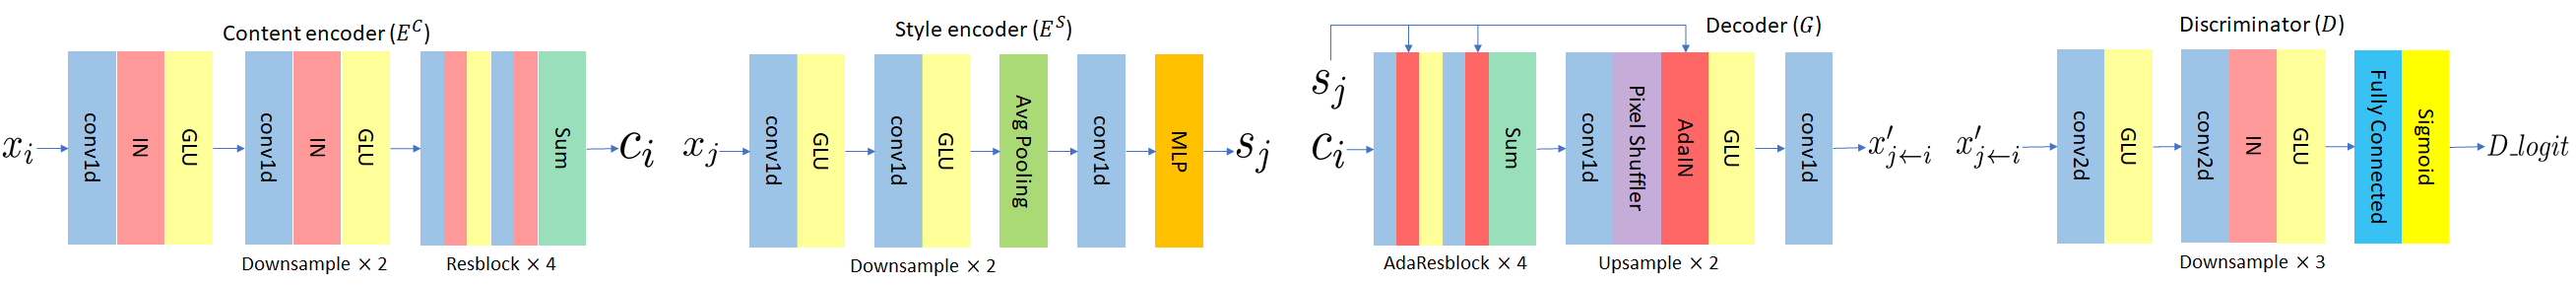
\includegraphics[width=1.0\textwidth]{FIG/NN}
\caption{The network architecture of content encoder, style encoder, decoder, and GAN discriminator.}
\label{fig:NN}
\end{figure*}

%It uses gated linear units (GLU) as activation function. The gating mechanism builds hierarchical representations of the input sequence. It takes $\mathcal{O}(N/k)$ operations to capture long-term dependencies of size $N$ (the kernel width is $k$), while recurrent networks need $\mathcal{O}(N)$ operations.
%encoding and decoding networks have mirror structure


\subsection{Objective evaluation}


\subsection{Subjective evaluation}
We conducted listening tests on Amazon MTurk to evaluate the converted speech \footnote{We provide converted samples at https://www.jian-gao.org/emovc}.


\section{Conclusion}
\label{sec:con}
We presented a nonparallel emotional speech conversion system. Objective and subjective evaluations showed that our model can successfully manipulate emotions to fool the emotion classifier as well as human listeners. As our approach does not require any paired data, transcripts or time alignment, it is easy to be applied in real-world situations. {\color{blue} One limitation is that the current model is restricted to one specific speaker.} Future work is to develop a general model that can do emotion conversion for unseen speakers. Additionally, we will build a larger database for training deep neural networks.

%We will continue to improve the speech quality.

%Future work includes using speech labeled in dimensional emotion space and control the degree of emotion.
%It is based on an autoencoder model where the speech signal is decomposed into an emotion-invariant content code and an emotion-dependent style code.
%to build a larger database. improve speech quality, train on multi

% To start a new column (but not a new page) and help balance the last-page
% column length use \vfill\pagebreak.
% -------------------------------------------------------------------------
%\vfill
%\pagebreak


%\section{REFERENCES}
%\label{sec:refs}
%
% \cite{C2}
%
%% References should be produced using the bibtex program from suitable
%% BiBTeX files (here: strings, refs, manuals). The IEEEbib.bst bibliography
%% style file from IEEE produces unsorted bibliography list.
%% -------------------------------------------------------------------------
\bibliographystyle{IEEEbib}
\bibliography{refs}

\end{document}




%1. An overview of voice conversion systems
%2. ACCENT CONVERSION USING PHONETIC POSTERIORGRAMS
%3. Wang, M., Wen, M., Hirose, K., Minematsu, N., 2012. Emotional voice conversion for mandarin using tone nucleus model–small corpus and high efficiency. In: Proceedings of the Speech Prosody
%4. Li, B., Xiao, Z., Shen, Y., Zhou, Q., Tao, Z., 2012. Emotional speech conversion based on spectrum-prosody dual transformation. In: Proceedings of the ICSP
%5. Wang, Z., Yu, Y., 2014. Multi-level prosody and spectrum conversion for emotional speech synthesis. In: Proceedings of the ICSP
%6. Voice conversion for emotional speech: Rule-based synthesis with degree of emotion controllable in dimensional space
%7. Kawahara, H., Masuda-Katsuse, I., De Cheveigne, A., 1999. Restructuring speech representations using a pitch-adaptive time frequency smoothing and an instantaneousfrequency-based f0 extraction: possible role of a repetitive structure in sound. Speech Commun. 27 (3), 187–207
%8. Fujisaki, H., Hirose, K., 1984. Analysis of voice fundamental frequency contours for declarative sentences of Japanese. J. Acoust. Soc. Jpn. (E) 5 (4), 233–242.
%9. A study on applying target prediction model to parameterize power envelope of emotional speech
%10. Image Style Transfer Using Convolutional Neural Networks
%11. Kawanami, H., Iwami, Y., Toda, T., Saruwatari, H., Shikano, K., 2003. Gmm-based voice conversion applied to emotional speech synthesis. IEEE Trans Speech Audio Proc. 7. pp. 2401–2404.

%13. Y. N. Dauphin, A. Fan, M. Auli, and D. Grangier, “Language modeling with gated convolutional networks,” in Proc. ICML, 2017, pp. 933–941.
%14. Unpaired image-to-image translation using cycle-consistent adversarial networks,
%15. Multimodal Unsupervised Image-to-Image Translation
%16. Generative Adversarial Nets
%17. C. Busso, M. Bulut, C.-C. Lee, A. Kazemzadeh, E. Mower, S. Kim, J. N. Chang, S. Lee, and S. S. Narayanan, “Iemocap: Interactive emotional dyadic motion capture database,” Language resources and evaluation, vol. 42, no. 4, p. 335, 2008.
%18. Voice Conversion from Unaligned Corpora using Variational Autoencoding Wasserstein Generative Adversarial Networks
%19 Unpaired image-to-image translation using cycle-consistent adversarial networks
%20. HIGH-QUALITY NONPARALLEL VOICE CONVERSION BASED ON CYCLE-CONSISTENT ADVERSARIAL NETWORK
%21. PARALLEL-DATA-FREE VOICE CONVERSION USING CYCLE-CONSISTENT ADVERSARIAL NETWORKS
%22. Voice Conversion from Non-parallel Corpora Using Variational Auto-encoder
%23. WaveNet: a generative model for raw audio
%24. Speaker-dependent WaveNet vocoder
%25. STARGAN-VC NON-PARALLEL MANY-TO-MANY VOICE CONVERSION
%26. Huang, C., Akagi, M., 2008. A three-layered model for expressive speech perceptionh. Speech Commun. 50 (10), 810–828
%27. M. Morise, F. Yokomori, and K. Ozawa, “WORLD: A vocoder-based high-quality speech synthesis system for real-time applications,” IEICE Trans. Inf. Syst., vol. 99, no. 7, pp. 1877–1884, 2016
%28. Arbitrary style transfer in real-time with adaptive instance normalization. ICCV (2017)


%xx. M. Arjovsky, S. Chintala, and L. Bottou, “Wasserstein generative adversarial networks,” in International Conference on Machine Learning, 2017, pp. 214–223


